%A more indepth look at how the system is designed with UML- and class-diagrams. Directed towards developers. Start with subsubsection here.

A more indepth look at how the system is designed with UML- and class-diagrams. It is divided into two main sections for the server and clients. The client section contains the different clients. After that follows the server section that is divided into different parts that makes up the whole server. 

%\section{Clients}
%Here is an explanation of the  different client system designs.
\section{Desktop application}
The desktop client is constructed around the model-view-controller pattern. It
relies heavily on action events being performed in the graphical interface which
is then handled by the controller. The model is the part handling the
communication and the storing of important information such as ongoing downloads
and the user token (used for communication authorization). In
\refer{chap:des_appendix} a UML-diagram of the desktop client is presented. 

\subsection{View}
The view of the \appName\ Desktop client is constructed with tabs. There are 5 different tabs. These are Search, Process, Upload, Workspace and Administration.

Each tab in the view is represented by its own java class. The QuerySearchTab class which represents the search tab can display both a search view and a results view. It uses the QueryBuilderRow class to construct the rows in the query builder which is used to construct search queries. The QueryBuilderRow class represents a row in the query builder and each row is dynamic and can change accordingly to user interaction. The search results are also implemented in the QuerySearchTab and the results are displayed with the TreeTable class which is further described in the utilities section below.

The UploadTab Class represents the upload view of the GUI. It has functionality to both upload a file to an existing experiment (which is separately handled in the UploadExistingExpPanel) and to create and upload a new experiment.

The ProcessTab class represents the process view in the GUI. It contains a list where files to be processed can be stored and a large number of processing parameters which can be changed by the user. There process tab also contains a console for displaying direct feedback on processes and an area which contains the status of all current processes which are being handled on the server. The later can be updated manually with a refresh button.

The major part of the WorkspaceTab class consists of a TreeTable which holds all the experiments and the corresponding data which the user has added to the workspace. Then there is also five buttons implemented which allows the user handle the data in the TreeTable. These buttons are Remove from workspace, Delete from database, Upload to, Download and Process. The TreeTable view can be changed to a view which displays all current and completed downloads. This is made using a tabbed pane containing the TreeTable view and the Downloads view.

\subsection{Model}
The model part of the system contains methods for doing most of the logic in the system. For example there are methods for sending login requests and for downloading files. There are separate classes for downloading and uploading files as well as a class for regular communication with the server called Connection. New connections are created with the ConnectionFactory class. The model also acts a storage for importating information such as the user token and list of ongoing downloads and uploads.

The AnalyzeTab Class is not yet implemented.

\subsection{Requests}
The Request package contains the Request class , the RequestFactory and all the classes that extends the Request class. Request is the super class and can make a JSON package that all the other Request classes can use. All requests must have a name, type and an URL, but can consist of more information. For example LoginRequest also has username and password. RequestFactory is a class that can create all objects from all types of requests. It is a way to easily create all requests from the same place.


\subsection{Response}
This package consists of all types of responses that the server can send to the client-program. There is a class named Response that all the other response classes extends from. For example there is a response class for the login request called LoginResponse. All types of responses have different properties. There is also a class ResponseParser that can parse the responses so that the important information can be taken out of a JSON-package. This information can then be used to tell the client program what should happen next in the user interface.


\subsection{Controller}
The controller part of the system consists of ActionListeners for the different buttons and functionalities in the view. For example there are Listeners for searching, downloading and processing. The Controller class has access to both the view and the model and acts as a middle hand between those two parts of the system. Usually a Listener in the controller reacts upon user input and then modifies the model and gives information about the change to the view.


\subsection{Utilites}

There are several classes which represents different data in the system. There are classes for experiment data, file data and annotation data. For example when a search response is received from the server it is parsed into experiment data and the experiment data contains file data and annotation data. There is also a class representing Process feedback data.

The TreeTable class represents the table which displays experiment data, annotation data and file data in the Search and Workspace tabs. It is specially constructed to handle the data classes and it allows vertical sorting.

\subsection{System Administration}
%Till Sysadmin!
The system administration is developed separately from the rest of the GUI, and therefore has a slightly different way of communicating.

\textbf{Communication with the Server}


All communication between the server and the system administration tab follows a line of steps. See \refer{fig:adm_com_view} below.

\begin{enumerate}

  \item An event is triggered by the user clicking something.
  \item The listener for the active tab receives the event and sorts out which type it is, and calls the appropriate method in the \textit{SysadminController} class.
  \item The \textit{SysadminController} has the connection to the \textit{Model}, and calls the associated method there.
  \item The \textit{Model} creates the corresponding request for the server, and then creates a new connection.
  \item The \textit{Connection} receives the request from the \textit{Model} and sends the request to the server.


\end{enumerate}

If the event triggers a request for data, the \textit{Model} will use a parser to parse the data before sending it back to the GUI to present it to the user.


\begin{figure}[hbt!]
\addImage{adm_comm_view.png}
\caption{Communication Overview}
\label{fig:adm_com_view}
\end{figure}

\textbf{A communication example}

As a more detailed example of Figure \ref{fig:adm_com_view}. Assume that the user clicks the 'Genome Files' tab in the 'ADMINISTRATION' tab. This will trigger an event (1) to be handled by the \textit{SysadminTabChangeListener} (2) who will receive the event and execute the desired behavior of the tab, which is to directly show the available genome releases. This is done by sending a request to get available genome releases to the server and then parse the response. 

In order to contact the server the \textit{SysadminTabChangeListener} (2) calls the \textit{SysadminController} (3) who uses a reference to the class \textit{GenomeReleaseTableModel} (4) to call the method \textit{getGenomeReleases()}. \textit{getGenomeReleases()} will create a \textit{GetGenomeRequest} using the \textit{RequestFactory}. The request is then sent to the server through the \textit{Connection} class (5). The response from the server is passed to the \textit{ResponsParser} that parses the JSON respons into wanted \textit{GenomeReleaseData[]} object. The genome release array is return all the way back to \textit{SysadminController} (3) which updates \textit{GenomeReleaseTableModel} with the new \textit{GenomeReleaseData[]} and at last lets the GUI know that the data has changed through a new event (1). This will trigger the GUI to repaint and show the available data.

\textbf{Building the Administration Tabs}


All tabs under the Administration tab are built in a similar fashion and then added to a
JTabbedPane in the \textit{SysadminTab} class. Each tab has it’s own package containing 
all classes associated to the particular tab. All tabs are also built step by step by 
using smaller methods creating panels and components. Each tab has at least one main 
listener that is added to all components that require listeners. Once an event is triggered 
in a tab the corresponding listener simply use a switch case based on button/tab names 
to decide which action to take. The main listeners have an instance of the \textit{SysadminController }
to be able to further handle requests from the user and send them forward to the \textit{Model} if neccessary.

\textbf{Important classes}
The system administration part of the desktop application depends on quite a few classes and is based loosely on the model-view-controller design pattern. Here follows a list of the most important classes and a short desciption of their function and responsibilities.
\begin{itemize}
\item SysadminController - Handles the communication between the SysadminTab and the GenomizerModel. The SysadminController creates all ActionListeners for the buttons in the different views. Some minor commands are handled within the sysadmin package, but user commands requiring input or output from the server are recieved from the different components of the SysadminTab and sent to the GenomizerModel which converts them to Request objects and sends them on to the server.
\item SysadminTab - Builds all of the different views that are displayed within the system administration tab. When creating the views it also adds the ActionListeners to the buttons and fields. It also holds a reference to all of the view components it has created so that information can be sent to and from the controller when needed.
\item The listener classes - These are added to all of the components of the view that the user can interact with. When an action is performed, the listener performs the action that is assigned to the command string associated with the action. All of the command strings are stored in the SysStrings class for easy access.
\end{itemize}


\textbf{Button and Tab names}

To simplify the naming of buttons and tabs a class called SysStrings is used. All buttons or tabs are named here and then this class is used when setting the actual names. This is to avoid hard code as well as making names easy to change and hence more dynamic.

\subsection{Flow of the system}

The sequence diagram in \refer{fig:des_download-sequence} describes the flow of the system when the user presses the download file button and the diagram in \refer{fig:des_login-sequence} describes how the desktop clients reacts to a login.

\begin{figure}[htb!]
	\addImage{des_download-sequence.jpeg}
	\caption{UML sequence diagram of downloading a file}
	\label{fig:des_download-sequence}
\end{figure}

\begin{figure}[htb!]
	\addImage{des_login-sequence.jpeg}
	\caption{UML sequence diagram of login}
	\label{fig:des_login-sequence}
\end{figure}
\FloatBarrier

\FloatBarrier

\section{Web application}
This section describes the design of our system, first with a system overview and then with more indebth information about our tabs.
\subsubsection{How our web application works}
%figure x5
\begin{figure}[h]
\centering
\includegraphics[width=1\textwidth]{web_system_backboneWebapp.png}
\caption{\label{fig:web_system_backboneWebapp}A general build of a backbone webapp.}
\end{figure}

\refer{fig:web_system_backboneWebapp} shows how a backbone\cite{web_1} web application works in general. We have a user, that interacts with a browser. A browser renders the DOM of our web application. How it does this is up to the browser. Different browsers might display it differently. Models and Collections will talk to the server to update themselves. For example, our \textit{Experiments} collection will retrieve experiments from the server and update itself with a call to it’s fetch() method. Out of the components that go into this figure, we are in charge of and only capable of changing a few of these; \textbf{View}, \textbf{Template}, \textbf{Collection} and \textbf{Model}. See the Backbone section of Frameworks in section \ref{sec:web_frame} more information.

\subsubsection{System overview}
%figure 2
\begin{figure}[h]
\centering
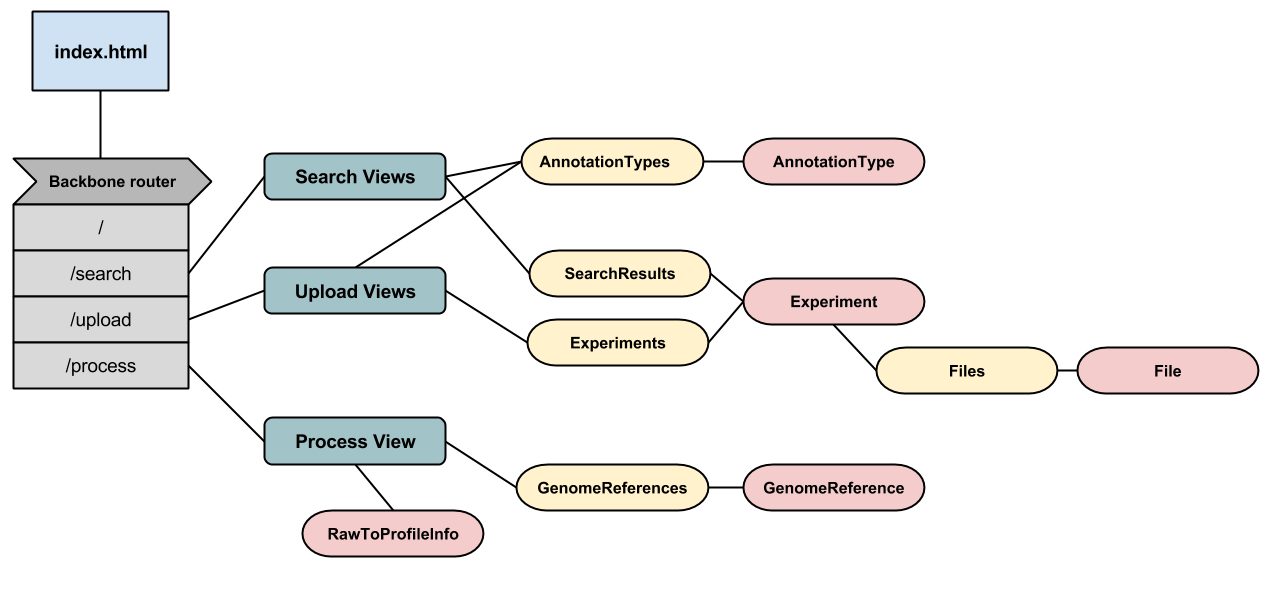
\includegraphics[width=1\textwidth]{web_system_overview.png}
\caption{\label{fig:web_system_overview}Overview of the relations between the different javaScript prototypes in the system.}
\end{figure}

Since our app is built using Backbone\cite{web_1}, our app is divided into the parts \textbf{Misc}, \textbf{Views}, \textbf{Collections} and \textbf{Models}. In \refer{fig:web_system_overview}, we can see the system overview. The \textbf{views} are the parts in green, the \textbf{collections} the parts in yellow and the \textbf{model} the parts in red. The parts in grey represent the router which belongs in our Misc category. It is responsible for rerouting links. For example, when a user clicks the search tab, the router navigates to /search, but instead of loading the whole /search over the page we are currently on, our router will open our search tab below our navigation bar. The \textbf{Misc} category also holds our Main.js, which is in charge of setting up and starting the app.

\subsubsection{Search}
The search tab has three views, the main one being \textit{Search}, which acts as a container for the \textit{SearchResultsView}and holds the search input field and the various buttons displayed. The \textit{SearchResultsView} handles rendering the annotations and the \textit{ExperimentViews}, where one \textit{ExperimentView} is created for every experiment returned from a search. The actual data retrieved is stored, by experiment, in \textit{Experiment models}. To organise this data, we have a collection to contain all the experiments retrieved, called \textit{SearchResults}.
 
%figure bla bla/lalalallala
\begin{figure}[h]
\centering
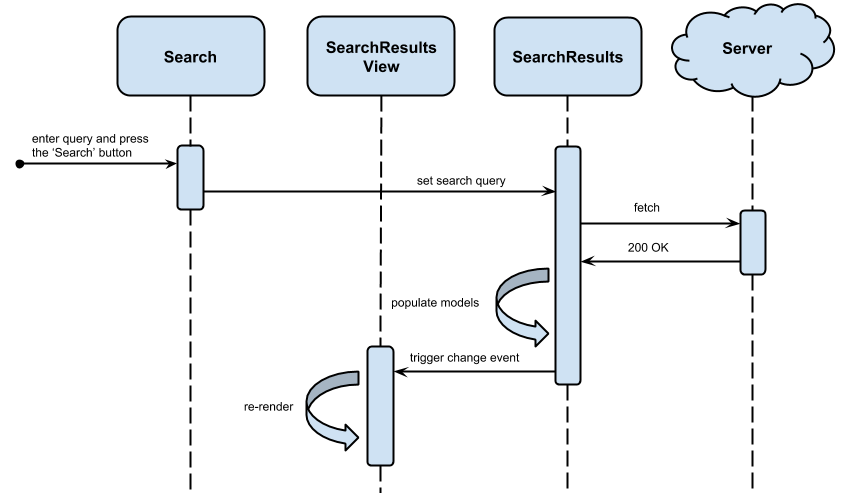
\includegraphics[width=1\textwidth]{web_system_sequenceDiagram.png}
\caption{\label{fig:web_system_sequenceDiagram}a sequence diagram showing what happens when a user enters a valid search query and results are fetched.}
\end{figure}

In \refer{fig:web_system_sequenceDiagram} is a simple sequence diagram for the search tab. If a user enters a query in the search field and then presses the search button, the \textit{Search} view will update the \textit{SearchResults} collection to have a new query. Once \textit{SearchResults} has a new query, it will try to fetch search results corresponding to the query from the server. If successful, new experiment models for every experiment retrieved will be created and set in the \textit{SearchResults} collection. \textit{SearchResults} then triggers a ‘change’ event that \textit{SearchResultsView} listens to. When that event occurs, \textit{SearchResultsView} knows that \textit{SearchResults} has been changed, and re-renders itself.


\subsubsection{Upload}
The upload tab has three main views, the main one being Upload, which acts as a container for the ExperimentView’s and holds the search input field and the various buttons displayed. Each ExperimentView handles rendering the AnnotationsForm and the FileUploadList, where one ExperimentView is created for every experiment the user inputs. The actual annotation data is stored by the \textit{Experiment} model. Files are stored as a \textit{Files} collection in the \textit{Experiment} model. \textit{Experiments} are in turn stored in the \textit{Experiments} collection.
\subsubsection{Process}
Processing has genomeReferences to match with the specie the processing is being done on. Other that that the processing part is mainly a graphical interface with not that much systemDesgin in.

\subsection{System administration - Web}
The system administration part of the web client is developed using the same tools and frameworks as the rest of the web client.
This admin part of the system is made up of view classes, model classes and collection classes. The classes are described below:

\subsubsection*{Classes used by all views}

\strongTerm{Gateway} - this is a model class used solely for communication with the server. It is a static class in the sense that it doesn't have to be created. It only needs to be included and then its functions can be called immediately without having to be instantiated. The gateway class retrieves the URL from the main JavaScript file this way the URL only needs to be declared once. The URL can then be fetched by any class that includes the Gateway class.

\strongTerm{SysadminMainView} - the main view for the admin tab, this view is used together with every other admin view. It contains a sidebar menu used to navigate between different admin views.

\subsubsection*{Classes used to handle annotations}

\strongTerm{Annotation} - this is a backbone model that represents an annotation. An annotation consists of three fields. A name, a list of values and a forced field. The name simply specifies the name of the annotation. The list determines whether this annotation is a drop-down list, or a free-text field. If the list contains one element called free-text, the annotation is a free-text field. Otherwise it is a drop-down list with the values in the list. The forced field determines if
the annotation has to be filled in by the user when a file is uploaded.

\strongTerm{Annotations} - this is a backbone collections that consists of several Annotation models. It also has a URL that it uses to fetch annotations from the server, the URL is retrieved from the Gateway class. 

\strongTerm{AnnotationsView} - this view is the basic view for displaying annotations. It has a search field and a button for creating new annotations. Pressing the button renders the newAnnotationView. 

The AnnotationsView has a child view called AnnotationListView. This way the list view can be rendered separately from the search field when the user types in searches. 

\strongTerm{AnnotationListView} - this view uses the Annotations collection to fetch all the annotations from the server and renders them dynamically in a list.
In the list is an Edit button for every annotation, the edit button will retrieve the name of the desired annotation and navigate through the router to the EditAnnotationView with the name as a parameter.
The view also has a button that will take the user to the NewAnnotationView.

\strongTerm{EditAnnotationView} - this view uses the name parameter received from the AnnotationListView to retrieve a specific annotation from the collection of annotations. It then renders the fields with the values from the annotation. This view has a button to delete an annotation. It will send a delete message to the server using the Gateway model to delete the annotation. An annotation can also be modified in different ways.

\strongTerm{NewAnnotationView} - this view is used to create a new annotation. It consists of a couple of fields and a create button. Pressing the create button renders a ConfirmAnnotationModal which displays the values for the annotation.

\strongTerm{ConfirmAnnotationModal} - this class extends the ModalAC class. It is simply used to display information that the user has to confirm. Pressing confirm creates a message using the Gateway class and sends it to the server.

\subsubsection*{Classes used to handle genome releases}

\strongTerm{GenomeReleaseView} - this view is used for viewing, adding and deleting genome releases. It contains a button ''Select files to upload'' which opens up file explorer and lets the user select one or multiple files for uploading. When the user then presses upload the UploadGenomeReleaseModal will open. Below the button the view has a table showing the current genome releases available on the server. The user can hold the mouse over files too see all files included in that genome release. A ''Delete'' button is shown next to every genome release and if pushed sends a delete request to the server through the Gateway class. 

\strongTerm{UploadGenomeReleaseModal} - this modal shows the user which files has been selected for upload and asks for information about which species and genome version they are for. Then at the press of ''Upload'' the files starts to upload and the user will see a progress bar over the complete upload progress. 

\strongTerm{GenomeReleaseFiles} - this is a collection with GenomeReleaseFile as models. It handles the ordering and filtering of its models. 

\strongTerm{GenomeReleaseFile} - this model represent a genome release and can contain multiple files in itself since one genome release is almost never just one file. This class takes case of uploading itself to the server and thereby also updates the progress bar through events that propagate up to the GenomeReleaseFiles collection. 

\FloatBarrier

\section{Android application}
The following sections describe the system design of the Android application. All functionality of the system components are described in this section. Worth noting is that the figures referred to in this section can be found further down in the document.

\subsection{System overview}
	The Android application is divided into seven \emph{packages}. These packages are \verb!default!, \verb!com!, \verb!login!, \verb!model!, \verb!process!, \verb!processStatus! and \verb!search!.
	All packages (except for \verb!com! and \verb!model!) contains one or several fragments. A \verb!Fragment! is an object that helps to modularize the code and brings more sophisticated user interfaces.

	\begin{figure}[h]
		\centering
		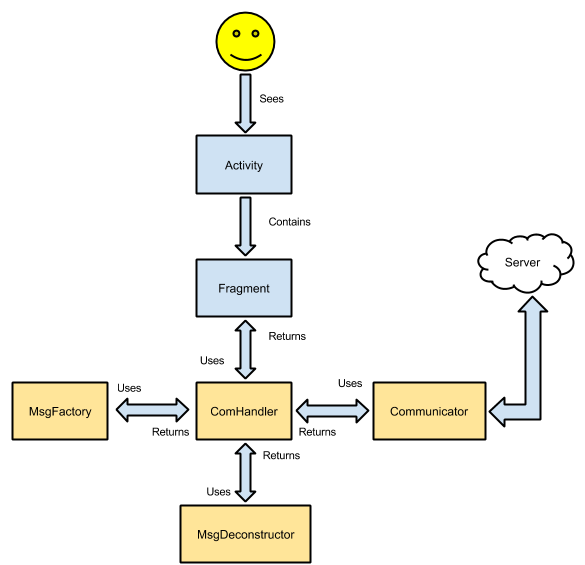
\includegraphics[width=1\textwidth]{and_system_overview.png}
		\caption{\label{fig:and_system_overview}A generalization of how the Android application works.}
	\end{figure}

	The user will interact with an activity that holds a fragment. The fragment (which contains some logic) will tell the class \verb!ComHandler! what action that should be performed. The \verb!ComHandler! will construct a message by using \verb!MsgFactory!. The message is then passed on to \verb!Communicator! which sends the message to the server with REST. The \verb!Communicator! returns the response to the \verb!ComHandler! that parses it by using the class \verb!MsgDeconstructor! and then returns it to the fragment. Hopefully, \refer{fig:and_system_overview} will bring some clarity.
	
\subsection{Package overview}
	The \verb!default! package contains the \verb!MainActivity!. This class is the base of every screen in the application after logging in. The top level navigation is handled from here.

	The \verb!com! package is responsible for communication with the server. It also contains classes and methods for construction and deconstruction of JSON.

	The \verb!login! package contains the GUI and controller for the login screen. It also enables the user to select, add, edit and delete server URLs.
	
	The \verb!model! package holds information about experiments, annotations, files etc. found on the server.
	
	The \verb!process! package is responsible for displaying processing parameters etc. for when the user wants to start a process.

	The \verb!processStatus! package shows the running, failed and succeeded processes on the server.
	
	The \verb!search! package handles searches by either selecting annotations, or by manually typing in PubMed style. It also handles the search results by displaying the found experiments in a list.
	
\pagebreak


\FloatBarrier

\section{iOS application}
The following sections describes the system design of the iOS application. The overall system design is discussed followed by a more detailed description of how the segues are controlled.

\subsection{Overall system design}
The  system is designed using the model-view-controller principle. Each view is controlled by its own controller class which reacts to user input and triggers changes in the model and updates the view accordingly.
\begin{figure}[ht]
\addScaledImage{0.3}{ios_UML2.png}
\caption{UML diagram.}
\label{fig:ios_UML}
\end{figure}
\FloatBarrier

\refer{fig:ios_UML} gives an overall image of the system design. Some classes are excluded from the figure to make it easier to get an overall idea of the system. The controller classes of the table cells and some other controller classes are not illustrated in the diagram. The non-excluded classes are described in \refer{table:ios_class_table}.

\begin{table}
\begin{tabularx}{\textwidth}{|l|X|}
\hline
\textbf{Class} & \textbf{Description} 
\\ \hline
\term{Annotation} &
Contains information about an annotation and can format the annotation name to an aesthetically more pleasing representation.
\\ \hline

\term{DataFileViewController} &
Controls the File view presented in \refer{fig:ios_files1}. It contains a reference to an experiment and lists all its files in a table.
\\ \hline

\term{Experiment} &
A class that contains information related to an experiment, as well as its files.
\\ \hline

\term{ExperimentDescriber} &
Generates a description of an experiment using annotations chosen by the user.
\\ \hline

\term{ExperimentFile} &
Contains information about a file from an experiment.
\\ \hline

\term{ExperimentParser} &
Parses experiment information from a NSDictionary to an Experiment object.
\\ \hline

\term{FileContainer} &
Contains files and sorts them by file type.
\\ \hline

\term{JSONBuilder} &
Creates different JSON requests.
\\ \hline

\term{PubMedBuilder} &
Creates a pubmed search query.
\\ \hline

\term{SearchResultController} &
A controller class for the Search Results view presented in  \refer{fig:ios_searchResult}. It configures the table which holds the information about the experiments a search resulted in. An ExperimentDescriber is used to generate a description of the experiments.
\\ \hline

\term{SearchViewController} &
A controller class for the Search view, see \refer{fig:ios_search}. It checks which annotation-fields are used and tells the JSONBuilder to generate a corresponding search query when the user presses the search button. The class also contains a advanced search to allow the user to manually enter search queries. 
\\ \hline

\term{SelectedFilesController} &
A controller class for the The selected files view shown in \refer{fig:ios_selectedFiles1}. The selected files controller contains information about files saved by the user.
\\ \hline

\term{ServerConnection} &
Sends and receives JSON objects to and from the server.
\\ \hline
\end{tabularx}

\caption{Description of some classes of the system.}
\label{table:ios_class_table}
\end{table}
\FloatBarrier

A more detailed description of these classes, and the ones not mentioned here, can be found in comments in the source code.

\subsection{Segue controll}
To avoid several segues to be executed at the same time, a segue controll package has been implemented. Instead of extending UIViewController, UITableViewController, UITabBarController and UINavigationBar the corresponding XYZ class should be used instead. An overview of this design can be seen in \refer{fig:ios_UML_segue}. This figure also includes the classes XYZDataFileController and XYZSearchResultController as two examples of such implementations.

\begin{figure}[ht]
\addScaledImage{0.35}{ios_uml_segue2.png}
\caption{UML diagram describing the segue controll.}
\label{fig:ios_UML_segue}
\end{figure}
\FloatBarrier


\FloatBarrier

\section{Server}
The design of the servers system is based around several parts. These parts consists of: communication, conversion, processing, storage and file transfer. Following is a more detailed description of each part.

\subsection{Communication}

\label{chap:com_systemdesign}
The server is based around a \texttt{RESTful} protocol where all communication is handled over non-persistent connections which the clients initiate. Since the communication is non-persistent, the server has no way of contacting clients except for responding to requests. When a client wants to connect it sends the request to a proxy, which only accepts encrypted trafic, that is then forwarded to the actual server. Once inside the server, the request is parsed, executed and a response is sent back to the proxy which forwards the message back to the client. 

To uniquely identify different logins a token is generated when a user logs in, the client now should identify itself with this token in all other requests for them to be executed. Otherwise, the server will not recognize who the client
is and therefore can't know what server commands the client has permissions to execute. 

Most commands are executed immediately when ther server recieves it, and the result is sent back as soon as the command is finished. There are however an exception to this, the process command, which is put in the back of a queue instead of being executed. The server continuously takes work from this queue and executes them as fast as it can, but due to the huge computing power requirement it cannot do them all at the same time. 

For a visual reference of the flow between the different parts of the system, see \fullref{fig:com_systemoverview}.

\paragraph*{Server Commands}

The following eleven items are the main categories of commands that can be sent: 

\begin{itemize}
	\item \textit{Connection}
	\item \textit{Experiment}
	\item \textit{Files}
	\item \textit{File conversion}
	\item \textit{Search}
	\item \textit{User}
	\item \textit{Admin}
	\item \textit{Processing}
	\item \textit{Annotation}
	\item \textit{Genome release}
	\item \textit{File upload/download}
\end{itemize}

Connection handles the \textit{Login} and \textit{Logout} commands, which are self-explanatory in their functions. There is also

\subparagraph*{Connection}

Connection handles the \textit{Login} and \textit{Logout} commands, which are self-explanatory in their functions. There is also a deprecated command which can be used, but should not, to check if the clients token is still valid or if it has expired. This was used before, but was deemed unnecessary due to this check happening on every other command as well. 

\subparagraph*{Experiment}

Used to create new experiments, update or delete existing experiments as well as retrieving information about specific experiments. Deleting or retrieving information only requires the experiments ID, whilst creating new or updating existing experiments require annotations to be specified as well.

\subparagraph*{Files}

Contains commands to create new file-posts, update or delete existing file-posts and retrieving information about specific file-posts, just as Experiment does for experiments, but for file-posts. A file-post is a database entry which keeps information about a file, as well as the path to the file. A file cannot be uploaded without having a matching file-post. When discussing files in general, file-posts and the file together will be refered to as a file. 

\subparagraph*{File conversion}

File conversion has a single command, which converts files from one file-format to another. The formats that can be converted from and to are: \texttt{.bed}, \texttt{.gff}, \texttt{.sgr} and \texttt{.wig}. 

\subparagraph*{Search}

Search is used for searching after experiments in the database, the search uses a PubMed-style query system which can be found and explained at \url{http://www.ncbi.nlm.nih.gov/pubmed}. All experiments that match the query are sent back to the client. No post-processing or ordering is done on the list ofexperiments by the server.

\subparagraph*{User}

Only contains two commands at the moment, update and retrieve information. Via the update command users can updates their password, name (fullname, not username) and email. Any other editing of users is done via the Admin category. 

\subparagraph*{Admin}

The Admin commands are the primary way of creating, editing and deleting users. Creating a new user requires a username, password, privilege level, name and email. To make editing and deleting easy to use there is also a command to get a complete list of all the usernames in the system, which together with the get user command from User, a client can get all the information about any user. 

\subparagraph*{Process}

In order to process files, the client can send a process command which is a collection of sub-commands, one sub-command for each step of the processing pipeline. Each of these sub-commands contain all the information they need to run and a list of infiles and outfiles. 

When a process command is executed, it executes the each sub-command in order. Since a sub-command might contain many input files and output files, it in turn executes on all the input files, producing all the output files before finishing, and thus, causing the process to be parallellized in each step, but each step is sequential in order.

Process also has commands to retrieve information about all the processes that are waiting, running or finished as well as canceling a running or waiting process. 

\subparagraph*{Annotation}

Annotation has two different sub-categories, annotation field and annotation value, the field is the name of the annotation and the value is the actual value. A annotation can only have a single field, but several values, and is displayed with dropdown menus in the clients. The reason for two different sub-categories is that both of the two need to be able to be created, edited, deleted separately. The retrieve only retrieves full annotations, i.e. both the name and all the possible values. 

\subparagraph*{Genome release}

Genome release is used to manage genome releases, works similarly to how file works, except a single genome release-post can have many files associated with it. 

A more detailed specification of the API can be found in \refer{chap:com_api}.

\FloatBarrier
\subsection{Data Conversion}
The \appName\ service needs to be able to convert, process and visualize data. This chapter explains how this is done in the system.

%\begin{figure}[h]
%\addImage{UMLFinal.png}
%\caption{Class-diagram  for Process}
%\label{con_UML}
%\end{figure}
	
The \texttt{RawToProfileConverter}, \texttt{Smooth}, \texttt{Step}, \texttt{Ratio} and \texttt{Bowtie} extends the \texttt{Executor} class. The different processing commands can only start the corresponding processing method on these Executors. 


\subsubsection{Executor}
The executor class, as seen in figure 5.2.1, is a abstract superclass that is an entity that is able to execute various commands. The executor class is able to run programs as well as scripts and shell commands. The commands are specified in the call to the methods in this class. \newline

\begin{tabularx}{\textwidth}{|l|X|}
\hline
\term{executeCommand} &

\term{executeCommand} is a protected method used in processing to make command line calls to external dependencies used
in the various processing steps. Firstly a \term{processBuilder} is used to ensure a safe way to execute commands, after 
that the working directory is set and the error output stream is merged with the standard output. After a command has been 
started the output stream is then recorded with the help of a Scanner object and a \term{stringBuilder} object. When the 
command has been executed the termination status is checked and the recorded string is sent back to the caller. The command 
to be executed is represented as an array of strings.
\\ \hline

\end{tabularx}

\subsubsection{RawToProfileConverter}
The purpose of the \term{RawToProfileConverter} class is that it will be used by
\term{RawToProfProcessCommand} and do all the steps in the process pipeline produce a \term{profile
file} in \term{.wig} format. These steps are done by calling external dependencies such as programs and scripts which are executed with methods that is extended from
\term{Executor} class. 
\subsubsection{Smoothing}
The term{Smoothing} class is used on a \term{profile file} to smooth down the tips, making the data result less jagged.
\subsubsection{Step}
The term{Step} class is used on a \term{profile file} to lower the file's resolution.
\subsubsection{Description of different scripts and processing steps}

\begin{enumerate}
\item \term{BowTie}: Uses the external dependency Java tool Bowtie. 
Support for Bowtie2 is implemented but not fully tested. 
Bowtie creates unsorted \term{.sam} files from \term{.fastq} raw files.
The files are created in a temporary folder with the name \filePath{result\_X}, where X is the ID of the current thread. 
All other folders created is placed inside the folder from where the files used where placed.

\item \term{sortSam}: Uses external dependency Picard and sorts the \term{.sam} file and creates a new \term{.sam} files, sorted by coordinates.
The files are saved in the same temporary folder as in the Bowtie step.

\item \term{RemoveDuplicates}: Uses the external dependency Python tool Pyicos.
Takes a sorted \term{.sam} file and produces a new \term{.sam} file with all duplicate reads removed.
It is optional to save this \term{.sam} file to the database but it is saved in the temporary directory in the mean time.

\item \term{Convert}: Uses external dependency Python tool Pyicos.
This is the final step of raw to profile conversion and uses Pyicos to convert a given \term{.sam} file to \term{.wig} file.
All intermediate files are removed except optionally the \term{.sam} file which can be returned together with the final \term{.wig} file. All saved files are moved to the given profile directory path.

\item \term{Smooth}: smooths the file and creates a large \term{.sgr} file,
converted the customers \term{Perl script} by following the algorithm they  sent
us. This makes it more efficient. Puts the files in a folder called
\filePath{smoothing}.

\item \term{Step}: Takes the smoothed \term{.sgr} file and takes samples from it
with a specified interval and creates a smaller \term{.sgr} file. If stepping is done the files will be placed in the same folder as the previous step.

\item \term{Ratio Calculation}: Creates four \term{.sgr} files with the
\term{Perl script}
provided by the customer. Puts the files in a folder called \filePath{ratios}.

\item \term{Smooth}: After the ratio calculation, smoothing needs to be done
again with different parameters. Puts the files in a folder called
\filePath{smoothing}
\end{enumerate}


\LTXtable{\textwidth}{system_design/SERV_systemServer_ProcessingTable.tex}

\paragraph{BowTie}
BowTie takes a raw \term{.fastq} file together with a genome release and converts the \term{.fastq} file to a \term{.sam} file, which is the first step to make the desired \term{.wig} file.
After a \term{.sam} file is converted the external dependency \term{Picard} is run with its internal command \term{samSort}, which produces a sorted \term{.sam} file sorted by chromosome and position as needed to use the scripts.
\paragraph{After-processing scripts}
The different functions of the Perl scripts is explained below. They are explained in the same order that they are executed. All scripts take a directory of files to be processed as input parameter.
The given Perl scripts are modified and wrapped by expect scripts in order for better usability and callability from the Java implementation.
\subsubsection{Ratio calculation}
Does ratio calculation on the processed files, for each position in the IP sample with at least one mapped read, a ratio of IP - input (on a log2 scale) is calculated. If the read count in the input is below the read count mean (in the input sample) is calculated it is set to the mean ( or double mean (2 x mean) as user specified). If the input mean is below four the minimum input value is set to four (to avoid division by near zero values. Calculated as (read length x approximate total number of reads in input samples(9 millin))/ genome size (for Drosophila melanogaster 120381546)). A random number between -0.5 and 0,5 is added to the read counts before log2 conversion to make them discrete for statistical analysis. All ratio values are then adjusted by reducing each value by median of the ratios. This linear adjustment is carried out in order to compensate for differences in IP and input sequencing depth. Also, to visualize ratios distribution, ratios are plotted by binning ratios with user specified numbers of bins and minimum and maximum ratio values (200bins,minimum ratio value: -10, maximum ratio value:10). Ratio values are printed in sgr format.

\subsubsection{Smoothing and stepping}
Both Smoothing and Step are implemented as separate classes calling external Perl scripts.
The classes provide some validation and a clean interface towards the external dependencies.
The programs can handle file corruption to some extent. 
If the file contains empty or wrongly formatted rows the program will not crash, it will simply ignore the corrupt rows.

\paragraph{Smoothing}
Smoothing means that a trimmed mean value or median value for a position and its surrounding positions is calculated. The number of positions to smooth on is called the Window Size. For example: with a window size of 10, the smoothed value on position X is calculated on the interval (X-4, X+5). A number of position which below shouldn't be smoothed at all should also be provided. There's also one parameter called stepSize, if the stepSize is one the program will not do any stepping but if it's larger than 1 stepping will be done. Stepping is handled in this program by simply checking every time we are going to write to the new file if the current row's position is divisible with the stepSize, if it is we write to the file, otherwise the row is discarded.

\paragraph{Step}
Step also takes a window size, the number of genome reads to skip. 
This afterprocessing reduces the granularity of the file and thus the file size, whilst information is lost of course.


\paragraph{Tuple}
The tuple class is a data carrier that represents one row of data in an sgr file. It consists of the fields chromosome, position, signal and newSignal. Where signal is the signal-value read from the infile and newSignal is the updated value after smoothing have been done.
The methods in this class are all standard getters/setters except for the method toString which formats a row for the outfile and rounds of decimal numbers. The constructor is also of interest since it parse a row on tabs. Thus the fields in an infile needs to be seperated by tabs and not spaces. The constructor will throw an exception if the line it tries to parse is either null or if it does not consist of three columns separated by tabs where the first is a string and the second and third is a double.


\subsubsection{ProcessHandler}
The ProcessHandler is a controller that handles process-calls. Depending on the name of the process it handles it differently. It acts as an interface between the process-module and the rest of the program. 


\subsubsection{Logic \& interface}
The main logic in the ProcessHandler is a switch-case that switches on the name of the process being called. For example if the name of the process is “RawToProfile” is sets up a RawToProfile-converter and calls it. 

\begin{tabular}{|l| p{7cm}|}
\hline
processName & A string that tells the handler which kind of process should be
executed. \\ \hline
procedureParams & A list of string with the parameters to the different external
programs/scripts that will be called during the execution. The first element
will be a string with parameters/flags for the first external program that will
be called, and so on. \\ \hline
inFile & A string with a path to the directory containing the files that should
be operated on. \\ \hline
outFile & A string with a path to the directory where the result .sgr files
should be put. \\ \hline
\end{tabular}



:

\FloatBarrier
\subsection{File-transfer}
In the current version of the program the desktop clients and the web clients connect to different software on the server. The desktop clients connect directly to the server communication software whilst the web clients connect via the apache server and all non web requests that is to be calculated using the server software is automatically redirected by apache.
The redirect is setup in a way that all GET requests that have a /api/ tag in the URL will be redirected.
The exception for the desktop clients are file up- and downloads which are done through the apache server.

The download and upload will work for all platforms although this will not be implemented for Android and iOS clients due to hardware limitations.

If the client wishes to upload a file to the server they first send a request to the server-system which authenticates the client and stores the annotations for the file. The download and upload path is validated by the script to ensure that no invalid paths are sent to the scripts.

In \refer{fig:exp_flow} below it is shown how the systems handles the different types of messages the client-systems can send. The big square represents the Apache server with different parts of the Apache server within. The iOS and Android clients can only send some requests to the server-system. Meanwhile, the desktop client can send requests to the server-system and upload and download to/from the web server. The web client sends all its messages to the Apache server and if it is a request to do some sort of computation it will be redirected to the server-system and if it is a download, upload or web-page message it will be sent to the web server.

\begin{figure}[hbt]
\addImage{exp_flow}
\caption{The different types of messages sent between the systems.}
\label{fig:exp_flow}
\end{figure}

The current version of the system utilizes a file structure to organize HTML- and file requests on the server, the structure is illustrated in \refer{fig:exp_filestructure}. The Web-root folder contains the PHP-scripts for uploading and downloading files. The app folder contains the \appName\ web page. All folders of the experiments are located in the data folder, which contains folders for the different data-types.

\begin{figure}[hbt]
\addImage{exp_filestructure}
\caption{Illustrating the current file tree on the server machine.}
\label{fig:exp_filestructure}
\end{figure}
\FloatBarrier
\subsection{Data Storage}
In order to enable the annotation and subsequent searching for experiments and files the data stored on the server is complemented by a database of information. Each file uploaded to or generated by \appName\ belongs to an experiment which is identified by the experiment ID (expID). Each experiment created by the end user results in an entry in the database's \term{Experiment} table. Each experiment contains files that were either generated during the experiment (\term{raw} data) or processed from these files (\term{profile} or \term{region} data). The full database schema is shown in \refer{fig:dat_databaseSchema}.

\begin{figure}[p]
\centering
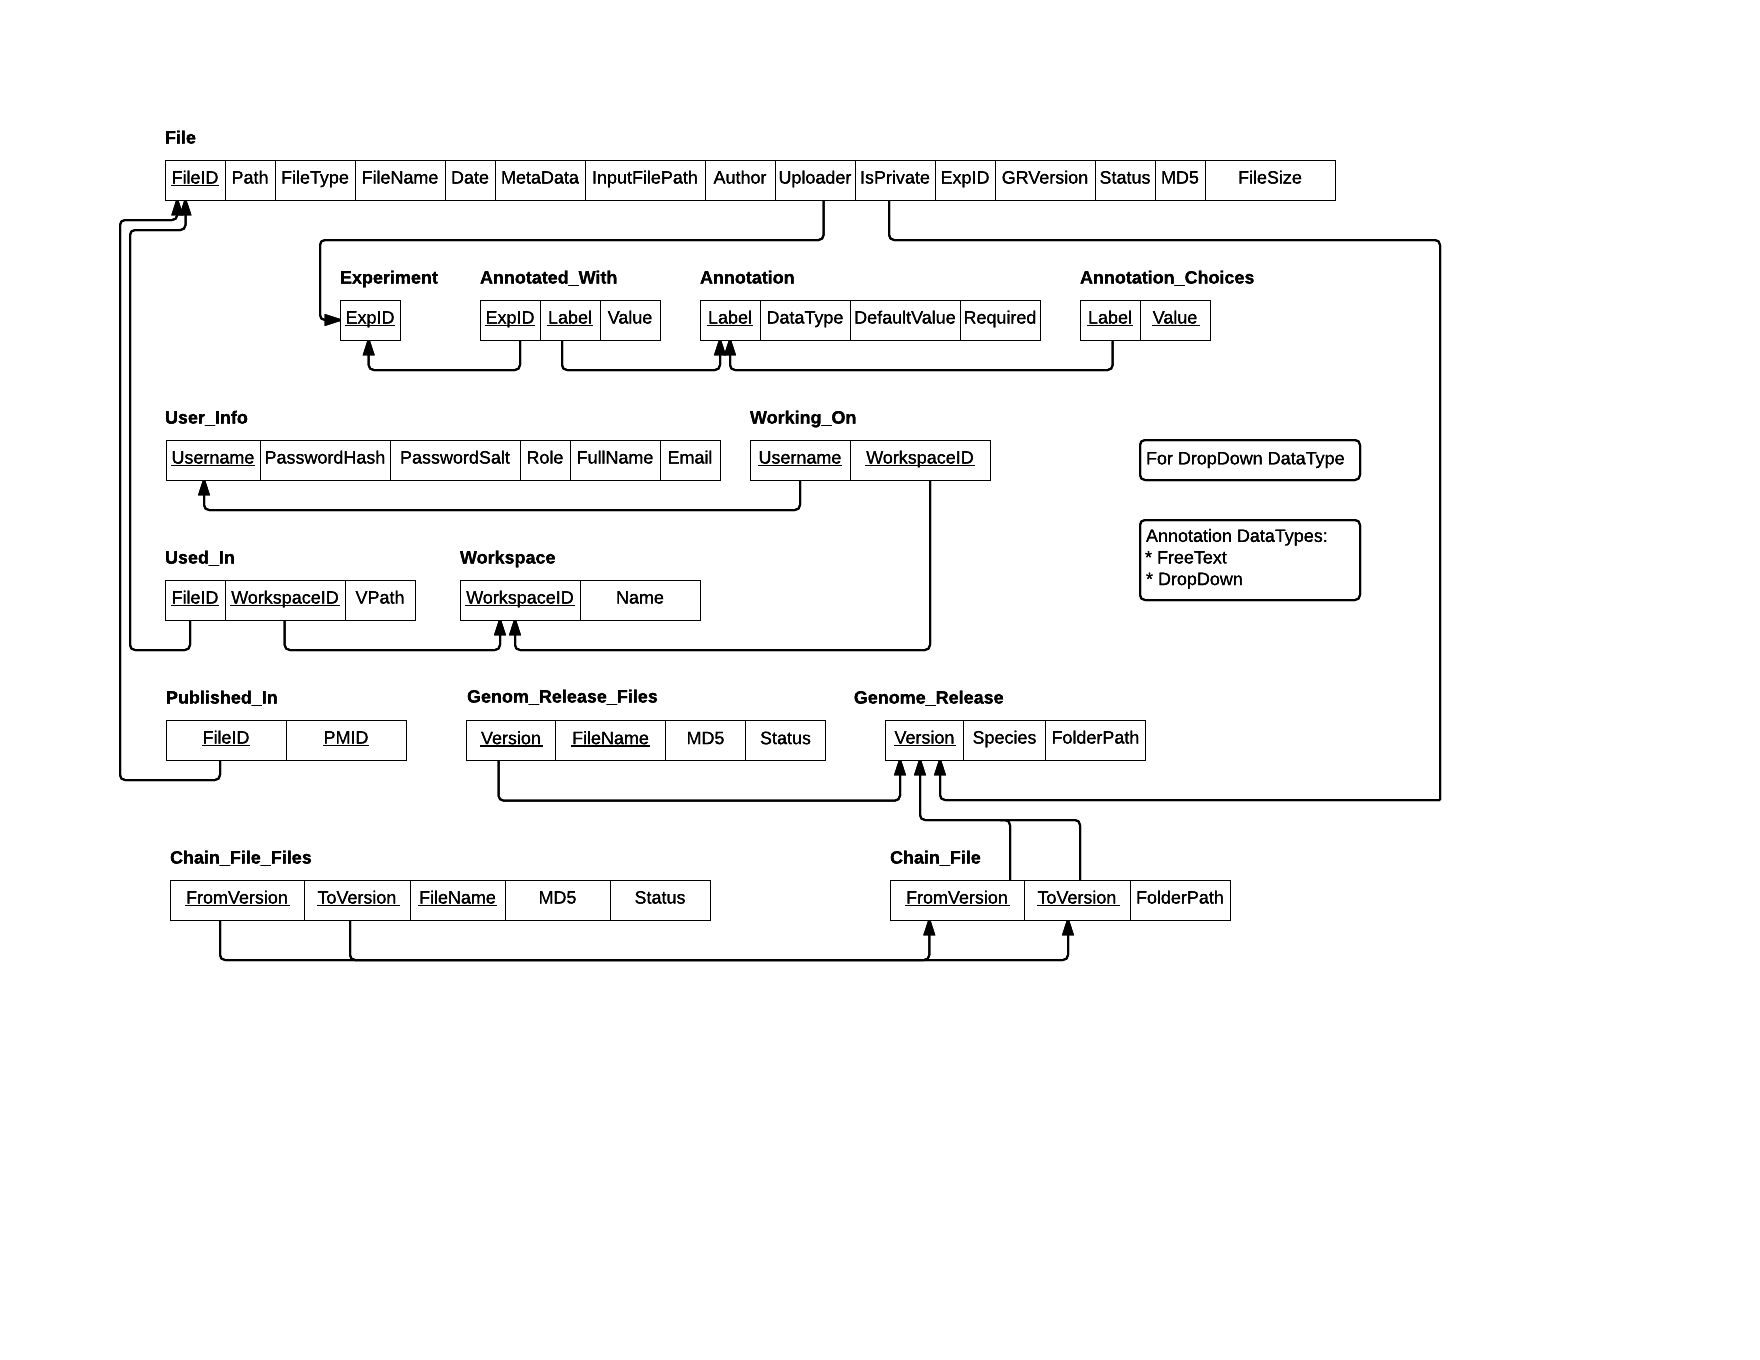
\includegraphics[width=20cm, angle=90, keepaspectratio=true]{dat_database_schema_v3.png}
%\addImageVertical{dat_database_schema_v3.png}
\caption{The database schema}
\label{fig:dat_databaseSchema}
\end{figure}

\FloatBarrier

\subsection{Database Design}
The following section will explain the less obvious columns and their intended use.

\texttt{FileID} is the identification number for a specific file. The data type \texttt{SERIAL} is used and will therefore be auto--generate unique identifiers upon insertion.

\texttt{Path} is the path to the corresponding file in the file system, for example: \\
\texttt{/var/www/data/Experiment1/raw/rawFile1.fastq}

\texttt{MetaData} is the string of parameters used in processing and should be \texttt{NULL} for all raw files.

\texttt{Annotated\_With} is the table that enables the annotation of experiments. The annotation in this table references the \texttt{Annotation}-table, to verify that new annotations are valid.

\begin{example}
To set the Species-annotation to ''Dog'' for the experiment Experiment1, the following tuple would be inserted into the Annotated\_With--table:
  \begin{center}
    \begin{tabular}{| l | l | l |}
      \hline
        \cellcolor{blue!25} ExpID & \cellcolor{blue!25} Label & \cellcolor{blue!25} Value \\
      \hline
      Experiment1 & Species & Dog \\
      \hline
      
    \end{tabular}
  \end{center}
\end{example}

\texttt{Annotation} is the table containing all the possible annotations a user can use to provide extra information about an experiment. This includes the type of annotation which is \term{Drop Down} for annotations where the user can choose from a drop down list, or \term{Free Text} where the user can enter the value freely. There is also support for a default value and annotation forcing where users are forced to provide the information. For \term{Drop Down} annotations the table \texttt{Annotation\_choices} specifies the valid choices.

The \texttt{Genome\_Release} table stores information about the \term{Genome Releases} available for use. This includes the unique version code for a \term{Genome Release}\cite{UCSCGRVERSION}. The \texttt{Genome\_Release\_Files} table stores the information about the files that make up the \term{Genome Release}.

\subsection{The Data Storage Subsystem}
All the classes used in the manipulation of the database and the creation of the file systems directory structure is contained in the java project's \texttt{database} package.

The other \appName\ subsystems execute all updates to the data storage through the \class{DatabaseAccessor} class. As a result there are many methods in this class, however most methods forwards the request to one of the classes in the \texttt{database.subclasses} package. Here the methods that modify the different areas of the data storage system are separated into different classes of more manageable sizes. An UML diagram of the \class{DatabaseAccessor} class and its subclasses is available in \refer{fig:dat_dbac} in  \refer{chap:dat_umls}.

The \class{DatabaseAccessor} utilizes a number of classes in order to return information to the method caller. These classes are contained in the \texttt{database.containers} package and are as follows:
\begin{itemize}
\item \class{Experiment}
\item \class{FileTuple}
\item \class{Annotation}
\item \class{Genome}
\end{itemize}

An UML diagram of these classes is also available in \refer{fig:dat_containers} in \refer{chap:dat_umls}.

\subsection{Interaction}
Below are examples of typical interactions with the \class{DatabaseAccessor} class.

\subsubsection{Adding an experiment}
In order to add an annotated experiment the following steps must be followed:
\begin{enumerate}
\item First the \term{addExperiment} method must be called. This will add one experiment to the database without any annotations set for that experiment. If you try to add one experiment that already exist then the addition will be refused and an exception will be thrown.

\item If there are no annotations that can be used to provide extra information about the experiment they must first be added by calling the \term{addFreeTextAnnotation} or \term{addDropDownAnnotation} methods.

\subitem If a \term{Drop Down} annotation already exists, but there is no suitable choice for the experiment a choice can be added by calling the \term{addDropDownAnnotationValue} method.

\item An available annotation can be used to provide extra information about an experiment by calling the \term{annotateExperiment} method.
\end{enumerate}

Now that an experiment has been added files can be added added to it.

\subsubsection{Annotation Handling}

Annotations can be handled using the methods below.

\begin{tabular}{|l| p{7cm}|}
\hline
\term{getChoices} & gets all the available annotation choices connected to a specific label. For example the possible choices returned for the label "sex" might be "Male, Female and Unknown". \\ \hline

\term{getAnnotations} & returns all annotation labels currently stored in the database. Examples could be "Sex,Species,Tissue,etc.". \\ \hline

\term{getAllAnnotationObjects} & Combines the two previous methods. Here an annotation object is returned that holds all the relevant information including the label, datatype, and the possible choices for a \term{Drop Down} annotation. \\ \hline

\term{changeAnnotationLabel} & updates the given label in the database. This will change the label for all experiments that use it. For example changing "specie" to "Species". \\ \hline

\term{changeAnnotationValue} & updates a value for a specific annotation label. For example changing "Human" to "Homosapien".  \\ \hline

\term{updateExperiment} & Updates an annotation for one specific experiment. Example: "experiment1, Species, Homosapien" can be changed to "experiment1, Species, Fly". \\ \hline

\term{deleteAnnotation} & deletes an unused annotation from the database. This will also delete all the choices for that annotation. \\ \hline

\term{removeAnnotationValue} & removes a single annotation value for a particular label. \\ \hline

\end{tabular}

\subsubsection{File Handling}
The actions of adding and deleting experiment files or genome releases can be performed using the following methods.

\begin{tabular}{|l| p{7cm}|}
\hline
\term{addNewFile} & To add a file you will need to have an experiment added before you call the \term{addNewFile} method. Raw files usually come in pairs and so they can be added together by specifying the input file name. \\ \hline

\term{deleteFile} & Deletes the given file from both the database and the file system. This can be done by either specifying the path or the file's ID number. \\ \hline

\term{addGenomeRelease} & Genome release files must be added one at a time by calling the \term{addGenomeRelease} method. This method returns an upload URL. \\ \hline

\term{removeGenomeRelease} & \term{removeGenomeRelease} removes all the files associated with a genome release. This can only be done if there are no files that have been generated using the specified genome release. \\ \hline
\end{tabular}
\FloatBarrier
